\chapter{Auswertung}
% =================================================================
\thispagestyle{fancy}
% =================================================================
\section{Gedämpfte Schwingung}
\subsection{Bestimmung der Eigenfrequenz}
Um die Eigenfrequenz zu bestimmen wurde jeweils zehn mal die Periodendauer bei vier verschiedenen Startauslenkungen gemessen. Dabei wurden sechs Magnete für die geschwindigkeitsproportionale Reibung verwendet. Die Messresultate sind im Anhang hinterlegt (Abbildung \ref{fig:messresultate_bestimmen_eigenfrequenz}).\\
\vspace{-0.4cm}
%%%%%%%%%%%%%%%%%%%%%%%%%%%%%%%%%%%%%%%%%%%%%%%%%%%%%%%%%%%%%%%%%%%%%%%%%%%%%%%%%%%%%%%%%%%%%%%%%%%%%%%%%%%%%%%%%%%%%%%%%%%%%%%%%%%%%%%%%%%%
\begin{figure}[h]
\centering
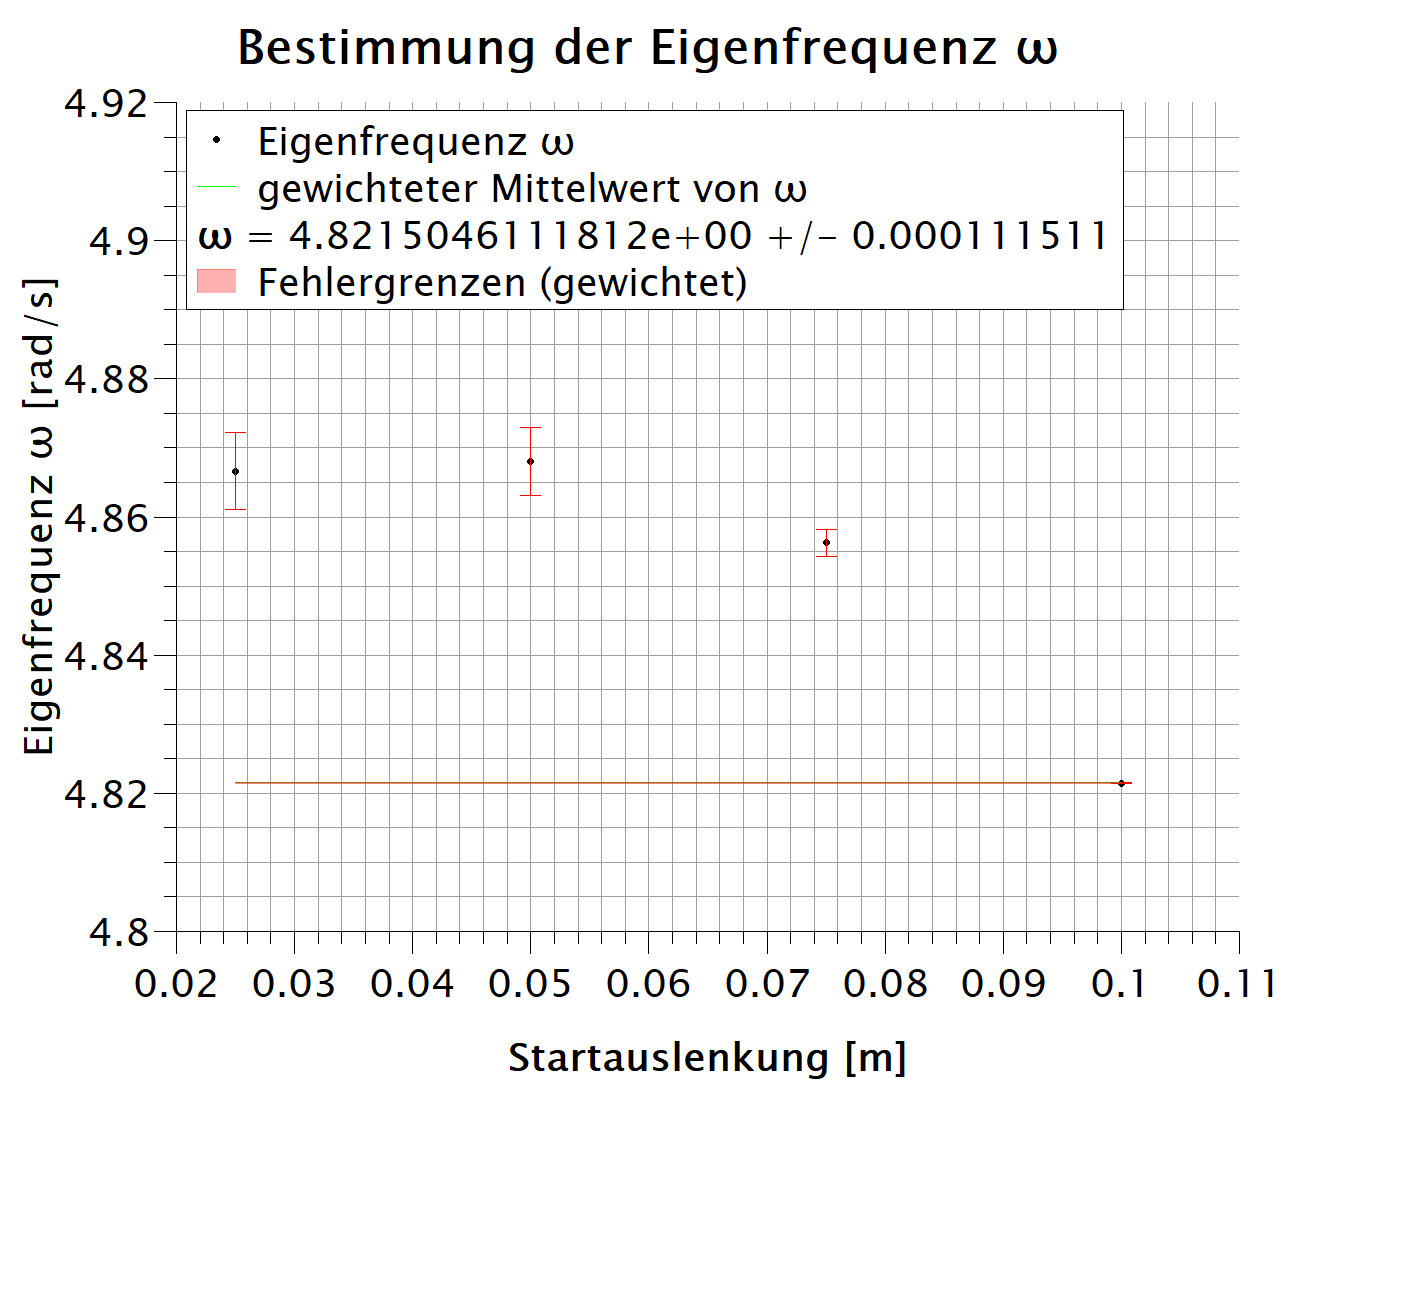
\includegraphics[scale=0.648]{Bilder/eigenfrequenz.png} 
\vspace*{-2.8cm}
\caption{Bestimmung der Eigenfrequenz mit vier verschiedenen Startauslenkungen. Deutlich zu erkennen ist, dass bei grösserer 					Startauslenkung der Fehler kleiner wird. Zur Berechnung von $\omega$ wurde der Kehrwert der gemessenen Periodendauer \textit{T} 		der Schwingung mit $2*\pi$ multipliziert. Davon der arithmetische Mittelwert und dessen ungewichteter Fehler berechnet. Diese sind dann, wie im Plot oben ersichtlich, mit den jeweiligen Fehlerbalken graphisch dargestellt. Anschliessend um eine möglichst genau angabe der Eigenfrequenz $\omega$ zu bekommen, wurde daraus der gewichtete Mittelwert mit dem gewichteten Fehler berechntet. (die Formeln dafür sind aus dem Kapitel 3.2 der Arbeitsunterlagen glaL3/glaL4 \cite{TechnikFHNW2016}). Da der gewichtete Fehler relativ klein erscheint, ist die grüne Linie des gewichteten Mittelwertes kaum zu sehen. }
\label{fig:eigenfrequenz}
\end{figure}
%%%%%%%%%%%%%%%%%%%%%%%%%%%%%%%%%%%%%%%%%%%%%%%%%%%%%%%%%%%%%%%%%%%%%%%%%%%%%%%%%%%%%%%%%%%%%%%%%%%%%%%%%%%%%%%%%%%%%%%%%%%%%%%%%%%%%%%%%%%%
\newpage
\subsection{Messung des Amplitudenverlaufs}
\label{subsec:amplitudenverlauf}
Der Amplitudenverlauf wurde viermal gemessen. Zweimal mit sechs Magneten und zweimal mit vier Magneten für die geschwindigkeitsproportionale Reibung. Dabei wurden wieder jeweils zwei unterschiedliche Startauslenkungen von $0.1m$ und $0.05m$ gewählt. Mit dem Laser Distanzmessgerät wurden die Positionsdaten des Fahrbahnpendels detektiert. In der Abbildung \ref{fig:amplitudenverlauf_01_6} einer der Amplitudenverläufe geplottet. Die anderen Verläufe befinden sich im Anhang (Abbildungen \ref{fig:amplitudenverlauf_005_4} \& \ref{fig:amplitudenverlauf_01_4} \& \ref{fig:amplitudenverlauf_005_6}). Die Messresultate befinden sich im Anhang (Abbildung \ref{fig:messresultate_amplitudenverlauf}).
\begin{figure}[H]
\centering
\includegraphics[scale=1.1]{Bilder/amplitudenverlauf_01_6.png} 
\caption{Startauslenkung von $0.1m$ mit sechs Magneten. $yd$ entspricht dabei dem \glqq genauen\grqq\: Wert der Startauslenkung.}
\label{fig:amplitudenverlauf_01_6}
\end{figure}
Anschliessend wurde aus den eruierten Daten $\omega_{0}$ mit dessen Fehler berechnet. Dafür muss die Gleichung \ref{equ:omega} nach $\omega_{0}$ umgeformt werden, woraus sich folgende Formel ergab:
\begin{equation}
\omega_{0}=\sqrt{\omega^{2}+\Gamma^{2}}
\label{equ:omega_0}
\end{equation}
Für jeden Run wurde dann $\omega_{0}$ mit dessen Fehler (durch das Fehlerfortpflanzungsgesetz \cite{TechnikFHNW2016}) berechnet und in einem Diagramm dargestellt. Eine detailierte Rechnung ist im Kapitel der Fehlerrechnung hinterlegt. Es wurde nur hier berechnet, da für die graphische Darstellung der Fehler von $\omega_{0}$ benötigt wurde. $\omega_{0}$ beschreibt die Kreisfrequenz eines \textbf{ungedämpften} Fahrbahnpendels bei gleichen Bedingungen \cite{w6}.
\newpage
\begin{figure}[h]
\centering
\includegraphics[scale=1.1]{Bilder/omega_0_fuer_alle_runs.png} 
\caption{Hier sind die Messpunkte der vier Runs, bei welchen eine unterschiedliche Anzahl an Magneten und Startamplituden verwendet wurden, graphisch Dargestellt. Es kann deutlich erkennt werden, dass die zwei Messpunkte auf der rechten Seite auf dem Bild eine höhere Kreisfrequenz $\omega_{0}$ aufweisen. Grund dafür ist, dass beim dritten und vierten Run nur vier Magnete für die geschwindigkeitsproportionale Reibung verwendet wurde. Bei den linken Messpunkten wurden dabei sechs Magnete verwendet. In diesem Falle entsprechen die Resultate den Erwartungen.}
\label{fig:omega_0}
\end{figure}
\newpage
\section{Erzwungene Schwingung}
\subsection{Amplituden- und Phasenresonanz}
Für die Bestimmung der Amplituden- und Phasenresonanz wurde das Fahrbahnpendel mit einem Schrittmotor angeregt. Dabei wurde mit einem Frequenzgenerator der Schrittmotor frequenzartig angetrieben. Dieser Motor drehte dann die Exzenterscheibe, von welcher die Periodendauer \textit{T} mit der Lichtschranke II)\footnote{veranschaulichung in der Abbildung \ref{fig:versuchsaufbau}} gemessen werden konnte. Der Kehrwert von \textit{T} entsprach dann der Erregerfrequenz. Die am Frequenzgenerator eingestellte Frequenz entspricht nicht der Erregerfrequenz, da diese nur dem Schrittmotor mitteilt, wieviele Schritte dieser pro Sekunde machen soll (ca. 1kHz bis 1.7kHz). Im Anhang, Abbildung \ref{fig:messresultate_phasenresonanz} sind die Messresultate hinterlegt.
\\[0.5cm]
Es wurde also eine Erregerfrequenz bestimmt und die daraus folgende Resonanz des Systems gemessen. Nach kurzem Einschwingen konnte mit dem Laser Distanzmessgerät die Amplitudenresonanz, sowie mittels Abgleichen der beiden Channels von der Lichtschranke I) und II) die Phasenresonanz für die unterschiedlichen Erregerfrequenzen gemessen werden. Für die Durchführung dieses Teilversuchs wurden zehn Magnete verwendet.
\begin{figure}[h]
\centering
\includegraphics[scale=1]{Bilder/amplitudenresonanz.png} 
\caption{Der Fit wurde anhand der Gleichung \ref{equ:erzwungene} gemacht. Allerdings musste wegen unbekanntem Gewicht $m$ des Fahrbahnpendels und Federkonstante $k_{1}$ die Gleichung mit $k_{1}/m=1/2*\omega_{0}^{2}$ angepasst werden. Somit konnten die Grössen $\omega_{0}$, $\Gamma$ und $\hat{y}_{e}$ eruiert werden.}
\label{fig:amplitudenresonanz}
\end{figure}
\newpage
\begin{figure}[h]
\centering
\includegraphics[scale=1.1]{Bilder/phasenresonanz.png} 
\caption{Die Phasenresonanz wurde nach der Gleichung \ref{equ:phasenresonanz} gefittet. Daraus ergaben sich die Grössen für $\Gamma$ und $\omega_{0}$ mit deren Fehler. Beim Fitten musste noch zusätzlich beachtet werden, dass der Tangens bei $90^{\circ}$ einen Pol hat, wodurch sich der Kosinus besser eignet. Es kann auch vermerkt werden, dass je näher die Erregerkreisfrequenz an die Kreisfrequenz $\omega_{0}$ kommt (also eine Phasendifferenz von $\pi/2$), desto höher wird die Amplitudenresonanz. Dieses Phänomen ist deutlich zu erkennen, wenn die Abbildungen \ref{fig:amplitudenresonanz} \& \ref{fig:phasenresonanz} miteinander verglichen werden.}
\label{fig:phasenresonanz}
\end{figure}